\section{Software Quality}


\subsection{Introduction}

\begin{frame}{Introduction}
\begin{itemize}
	\item Software has to fulfill certain quality criteria.
	\item Different domains can require different quality criteria.
	\item How bad is malfunction of the infotainment-system?
	\item How bad is malfunction of the ABS, which causes the wheels to block at full speed?
\end{itemize}
\end{frame}

\begin{frame}{Software Errors - Costs}
Study of Cambridge University (2012):
\begin{itemize}
	\item Software errors cost 320 billion Dollar per year.
	\item Developers spend 50\% of their time to find and fix errors.
	\item Costs will increase caused by increasing demand of software.
\end{itemize}
\end{frame}




\begin{frame}{Example - Mars Climate Orbiter}
\begin{columns}
\column{0.38\linewidth}
\centering
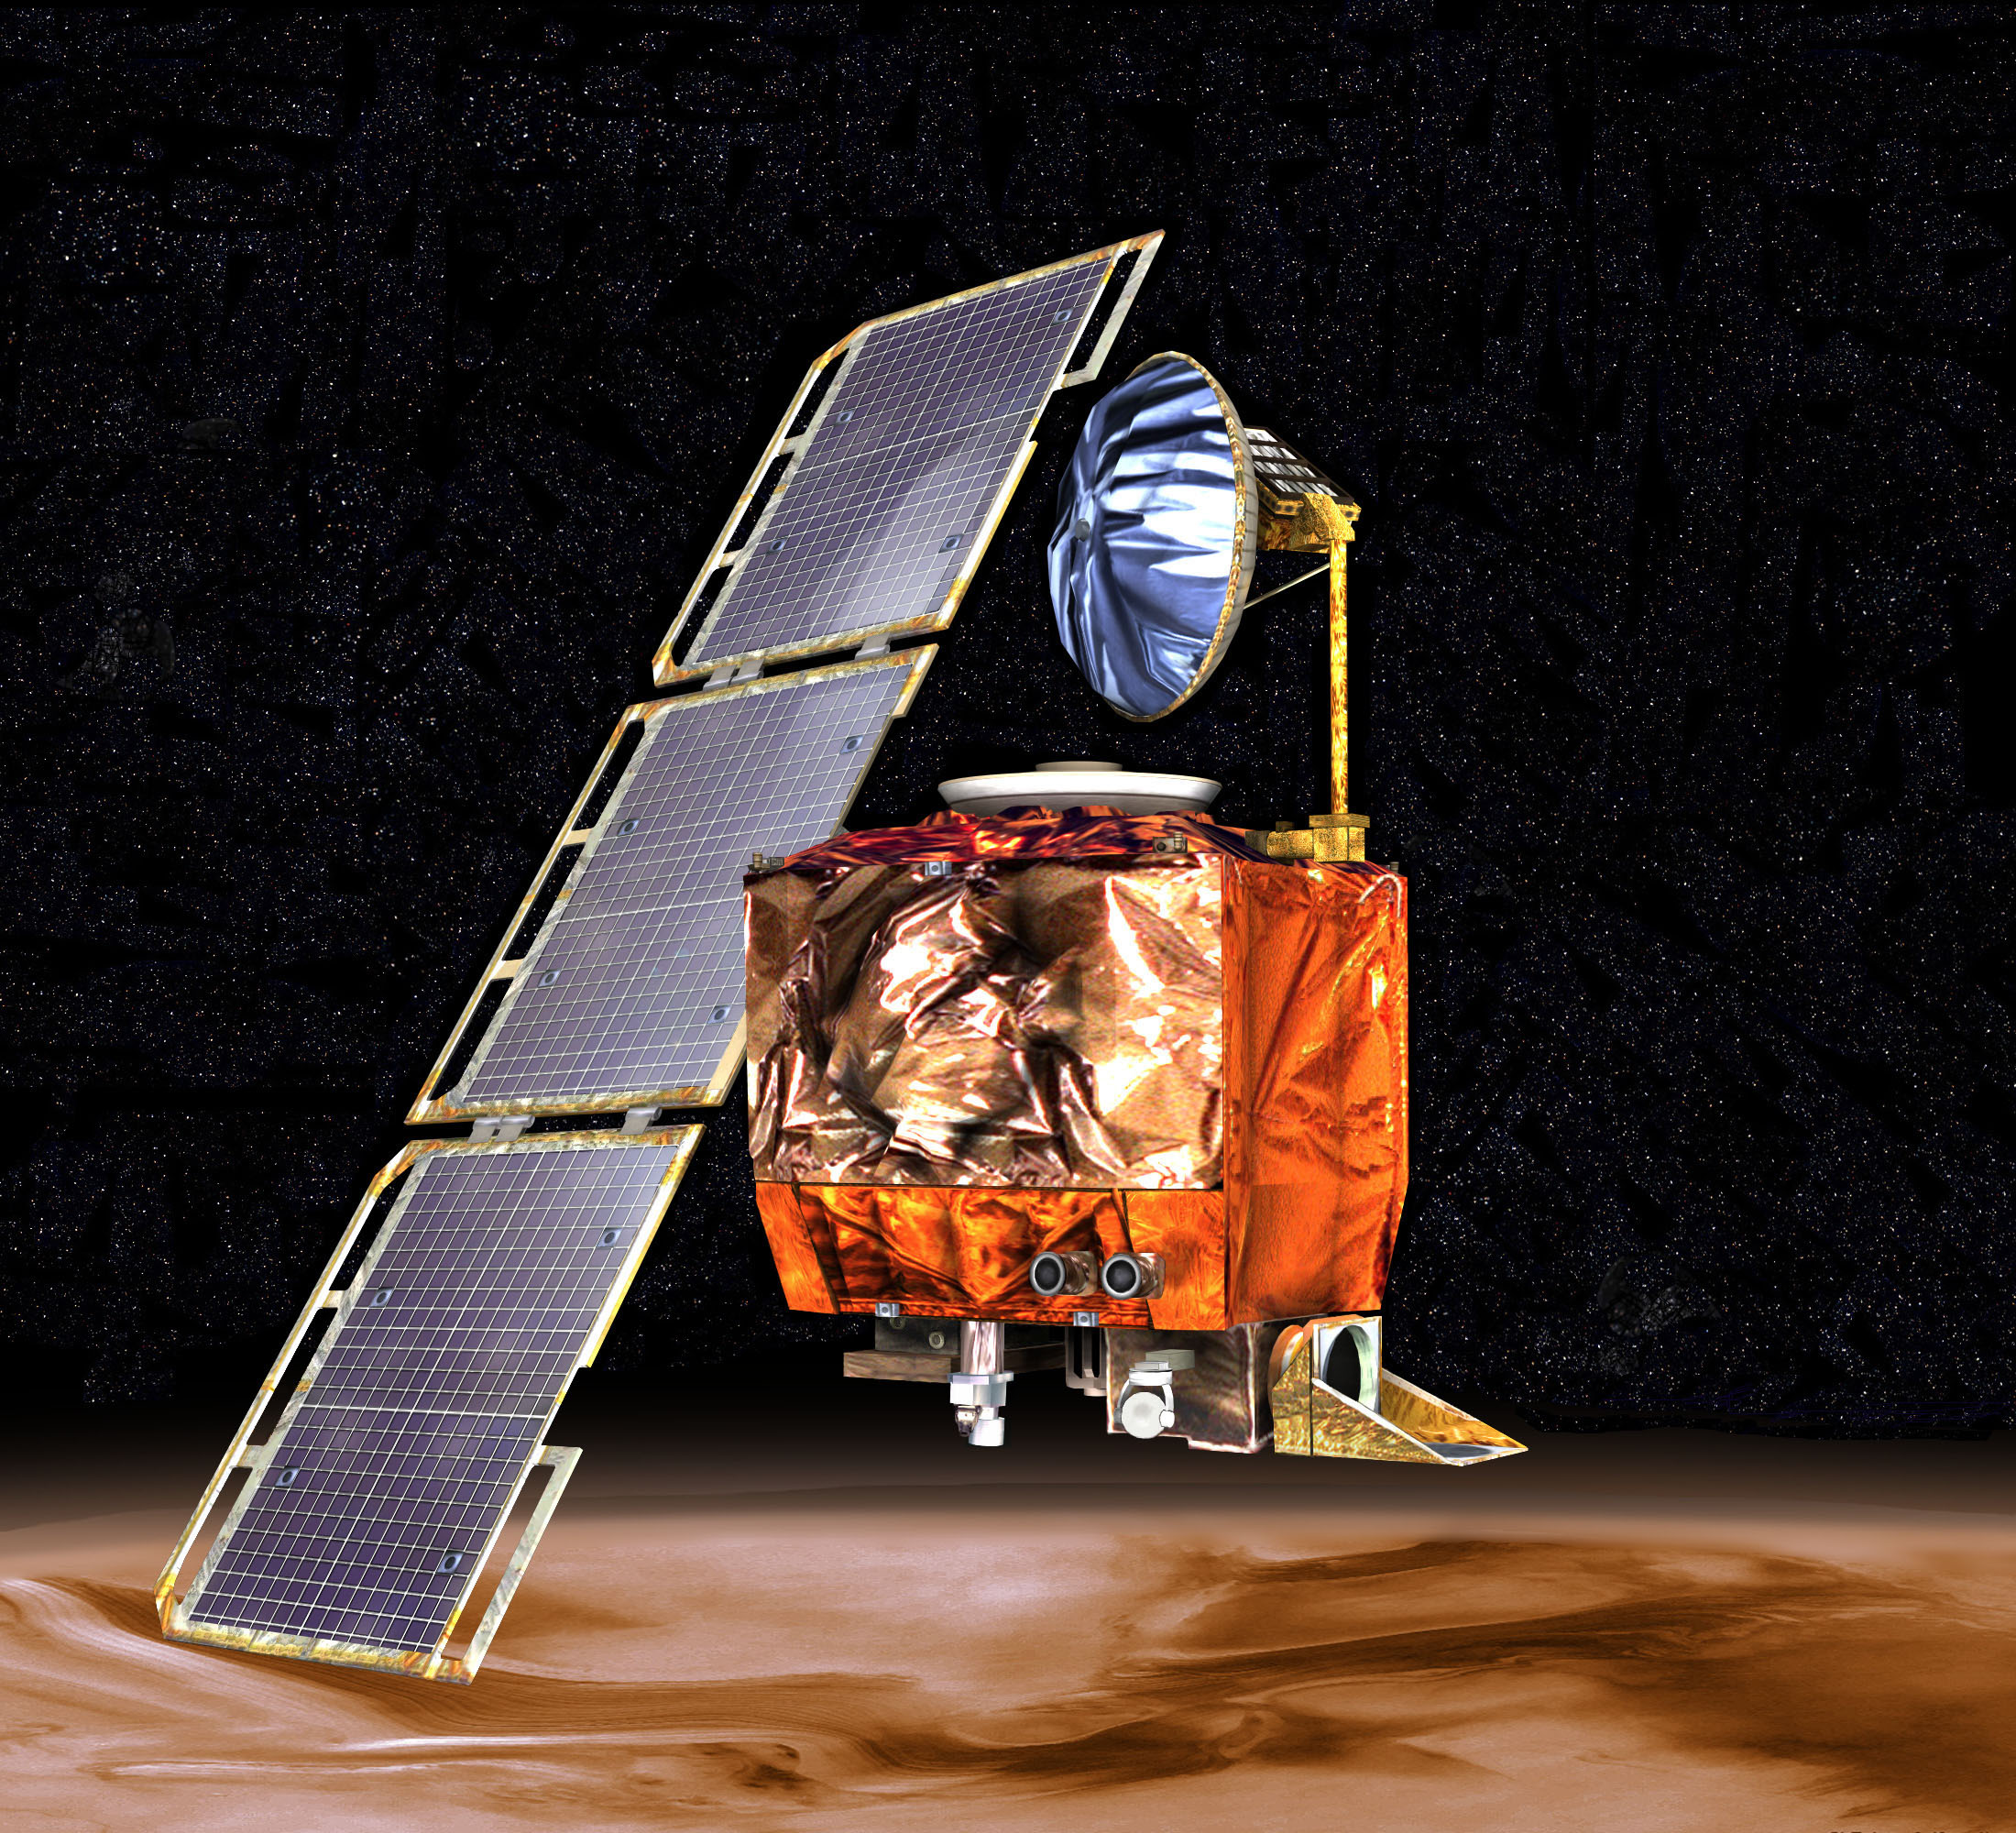
\includegraphics[width=\textwidth]{content/images/software-quality/mco.jpg}
\column{0.58\linewidth}
\begin{itemize}
	\item Mars Climate Orbiter was part of NASA's discovery program.
	\item Observation of the Mars surface from orbit.
	\item Communication-relay for other Mars- and Deep-Space-probes.
	\item Communication failed on 23.09.1992.
\end{itemize}
\end{columns} 
\end{frame}


\begin{frame}{Example - Mars Climate Orbiter}
\begin{itemize}
	\item Cause of failure: two teams participated to the software.
	\item One team calculated using the metric system, the other one with the imperial system.
	\item Therefore the MCO came to close to the Mars surface and burned in its atmosphere.
	\item Costs: about 194 Million USD
\end{itemize}
\end{frame}

\begin{frame}{Example - Mars Climate Orbiter}
\begin{figure}
\centering
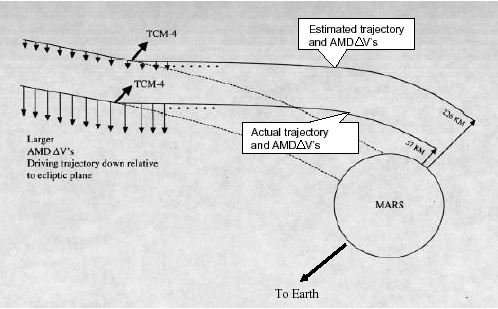
\includegraphics[width=\textwidth]{content/images/software-quality/mco_trajectory.jpg}
\end{figure} 
\end{frame}


\begin{frame}{Example - USS Yorktown}
\begin{columns}
\column{0.58\linewidth}
\begin{itemize}
	\item Cruiser of the US Navy
	\item In 1996 the ship was equipped with 27 workstations as part of the Smart Ship Project.
	\item The software indicated a closed valve as open.
	\item Correction by crew: Manual entry of a $0$ in a database.
	\item This lead to a division by $0$ and a total failure of al software systems including all engines.
\end{itemize}
\column{0.38\linewidth}
\centering
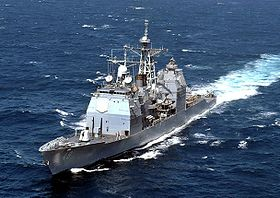
\includegraphics[width=\textwidth]{content/images/software-quality/yorktown.jpg}
\end{columns} 
\end{frame}




\subsection{Types of Errors}

\begin{frame}{Program errors}
\begin{minipage}[0.3\textheight]{\textwidth}
	\begin{columns}[T]
		\begin{column}{0.6\textwidth}
			\begin{itemize}
				\item Program errors are usually called \emph{bugs}.
				\item Usage of bug as synonym for program error was probably influenced by the computer scientist \emph{Grace Hopper}.
			\end{itemize}
		\end{column}
		\begin{column}{0.4\textwidth}
			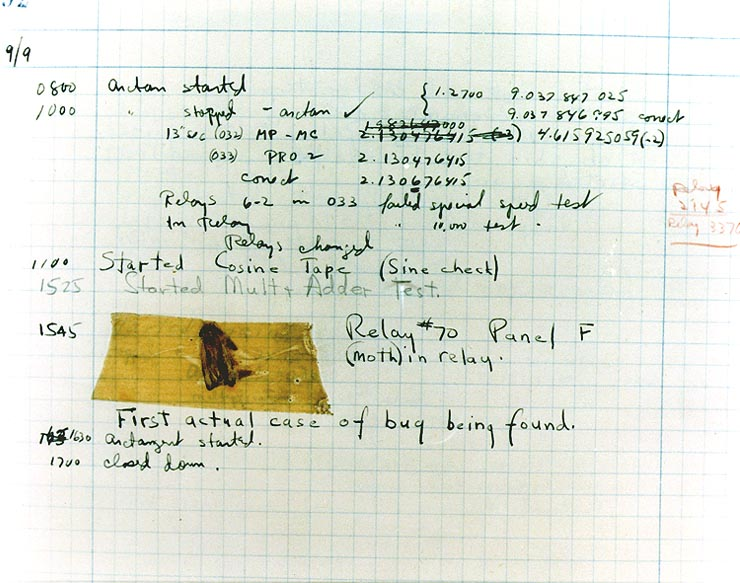
\includegraphics[width=\textwidth]{content/images/software-quality/bug.jpg}
		\end{column}
	\end{columns}
\end{minipage}

\begin{itemize}
	\item In the 1940s a moth was found in a relay of the computer \emph{Mark II Aiken Relay Calculator}, which led to a malfunction.
	\item The note \enquote{First actual case of bug being found} was written in the log and  the moth was pasted in.
\end{itemize}
\end{frame}

\subsubsection*{Categorization by IEEE}

\begin{frame}{Bugs}
\begin{block}{Bug - IEEE 610.12, 1990}
\textbf{bug.} \textit{See:} \textbf{error;fault.}
\end{block}
\begin{itemize}
	\item IEEE 610.12, 1990 \enquote{IEEE Standard Glossary of Software Engineering Terminology} defines various terms in the field of software engineering.
	\item According to the IEEE definition, the term bug comprises two parts: \emph{errors} and \emph{faults}.
\end{itemize}
\end{frame}

\begin{frame}{Error}
\begin{block}{Error - IEEE 610.12, 1990}
\textbf{error.} (1) The difference between a computed, observed, or measured value or condition and the true, specified, or theoretically correct value or condition.\\
(4) A human action that produces an incorrect result. For example an incorrect action on the part of a programmer or operator.
\end{block}
\end{frame}

\begin{frame}{Error}
\begin{itemize}
	\item In IEEE there are four different definitions for \emph{error}. 
	\item We emphasize on the fourth definition:
	\item An \emph{error} is a human mistake that causes a \emph{fault} .
\end{itemize}
\end{frame}

\begin{frame}{Fault}

\begin{block}{Fault - IEEE 610.12, 1990}
\textbf{fault.}\\ (1) A defect in a hardware device or component; for example, a short circuit or broken wire.\\
(2) An incorrect step, process, or data definition in a computer program.
\end{block}

\begin{itemize}
	\item In more general terms, a \emph{fault} is a deviation between the current and expected behavior of a system.
	\item Typically can \emph{faults} be detected by comparing the current and the expected state of the system.
	\item A \emph{fault} can cause a \emph{failure}, but must not necessarily.
\end{itemize}
\end{frame}

\begin{frame}{Failure}
\begin{block}{Failure - IEEE 610.12, 1990}
\textbf{failure.}\\ The inability of a system or component to perform its required functions within specified performance requirements.
\end{block}

\begin{itemize}
	\item A \emph{failure} can be seen by the deviation between the observed and the specified behavior of the system.
\end{itemize}

\end{frame}

\subsection{Classical Categorization}

\begin{frame}{Types of software errors}
A common classification of software errors comprises four categories:
\begin{enumerate}
	\item Syntax errors
	\item Runtime errors
	\item Logical errors
	\item Design errors
\end{enumerate}
\end{frame}

\begin{frame}[fragile]{Syntax errors}
\begin{itemize}
	\item Syntax errors are violations of the grammatical rules of the programming language.
	\item Syntax errors are detected by the compiler and cause the abortion of the compilation.
	\item In case of programming languages that are not compiled the program aborts during the execution.
\end{itemize}
\textbf{Example}
\begin{lstlisting}
int[] a = new int[10];
for (i = 0; i < a.length; i++) {}
\end{lstlisting}
\end{frame}

\begin{frame}[fragile]{Runtime errors}
\begin{itemize}
	\item Runtime errors include all types of errors that occur during the execution.
	\item Frequent runtime errors:
\begin{itemize}
	\item Exceeding the value range of a variable
	\item Iteration of arrays
	\item Insufficient checking of the user input
\end{itemize}
\end{itemize}
\textbf{Example}
\begin{lstlisting}
int[] a = new int[10];
for (int i = 0; i <= a.length; i++) {}
\end{lstlisting}
\end{frame}

\begin{frame}[fragile]{Logical errors}
\begin{itemize}
	\item Logical errors occur if the approach is wrong.
	\item Something wrong is calculated.
	\end{itemize}
	\textbf{Example - Summation of all integers between 1 and (including) 100}
\begin{lstlisting}
int sum = 0;
for (int i = 1; i < 100; i++) {
sum += i;
}
\end{lstlisting}
\begin{lstlisting}
int n = 100;
int sum = (n*(n+1)) / 2;
\end{lstlisting}
\begin{lstlisting}
int n = 100;
int sum = (n*(n-1)) / 2;
\end{lstlisting}
\end{frame}

\begin{frame}{Design errors}
\begin{itemize}
	\item Design errors are errors in the basic concept of the software.
	\item Possible causes:
	\begin{itemize}
		\item Wrong specification
		\item Inappropriate design of the software, i.e. for unexpected changes of the requirements
	\end{itemize}
\end{itemize}
\end{frame}


\subsection{Famous Errors}

\begin{frame}{Bohrbug}
\begin{itemize}
	\item There are certain types of errors, which have their own name.
	\item The Bohrbug was named after the danish physicist Niels Bohr.
	\item Niels Bohr developed the \emph{Bohr model} modeling the behavior of atoms as deterministic.
	\item A Bohrbug is deterministic and its behavior doesn't change by observing it.
\end{itemize}
\end{frame}

\begin{frame}{Heisenbugs}
\begin{itemize}
	\item The Heisenbug was named after the physicist Werner Heisenberg.
	\item Heisenberg introduced the uncertainty principle.
	\item A heisenbug is an error, that seems to disappear or changes its behavior, if the error is observed.
	\item Frequent cause: not initialized variables
\end{itemize}
\end{frame}

\begin{frame}{Mandelbug}
\begin{columns}
\column{.58\textwidth}
\begin{itemize}
	\item The Mandelbug was named after the mathematician Benoît Mandelbrot, who also gave his name to the Mandelbrot set.
	\item The cause of a Mandelbug is very complex and unexpected.
	\item A Mandelbug causes chaotic and unpredictable behavior.
\end{itemize}
\column{.42\textwidth}

\includegraphics[width=\textwidth]{content/images/software-quality/mandelbrot.png}
\end{columns}

\end{frame}

\begin{frame}{Schrödingbug}
\begin{itemize}
	\item The Schrödingbug was named after the physicist Erwin Schrödinger or after Schrödingers cat, respectively.
	\item A Schrödingbug is characterized by the fact, that the software seems to work flawless over a period of time until the error eventually occurs.
	\item The error is in a way that the software never should have worked.
\end{itemize}
\end{frame}

\begin{frame}{Hindenbug}
\begin{columns}
\column{.58\textwidth}
\begin{itemize}
	\item The Hindenbug is characterized by the fact, that its consequences are catastrophically.
	\item It was named after the zeppelin \emph{Hindenburg}.
\end{itemize}
\column{.42\textwidth}
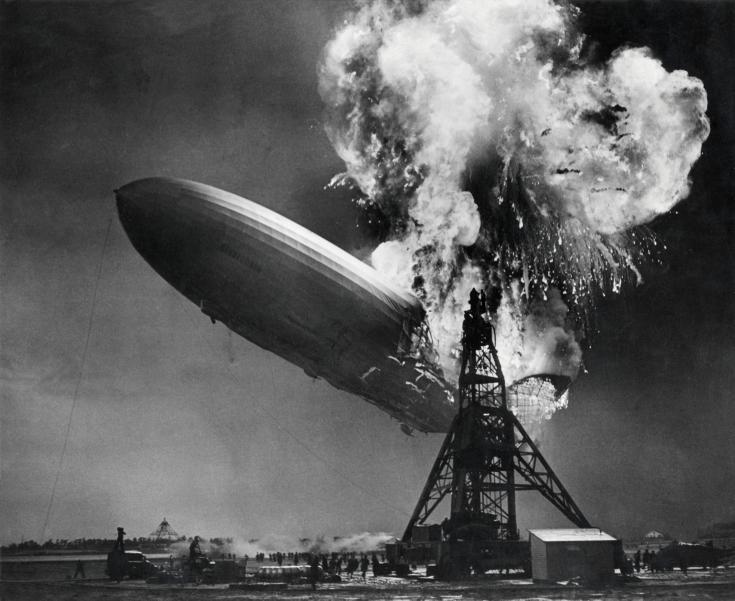
\includegraphics[width=\textwidth]{content/images/software-quality/hindenburg.jpg}
\end{columns}

\end{frame}

%aging bug

%Higgs bugson


\subsection{Quality Criteria}

\begin{frame}{What is quality?}
\begin{itemize}
	\item \enquote{Quality is the absence of unpleasant surprises.}
	
	\item \enquote{Quality is hard to define, impossible to measure, but easy to recognize.}
	
	\item \enquote{Quality is when the customer comes back and the product doesn't.}
	
\end{itemize}

\end{frame}


\begin{frame}{What is quality? (German Industrial Norm)}
\begin{block}{DIN 55350}
\textbf{Qualität --} Gesamtheit von Eigenschaften und Merkmalen eines Produktes oder einer Tätigkeit, die sich auf die Eignung zur Erfüllung gegebener Erfordernisse beziehen.\newline
\\
\textbf{Anmerkung 2:} Ein Produkt ist z.B. jede Art von Waren, Rohstoffen, aber auch der Inhalt von Konzepten und Entwürfen. Eine Tätigkeit ist z.B. jede Art von Dienstleistung, aber auch ein maschineller Arbeitsablauf wie ein Verfahren oder ein Prozess.\newline
\\
\textbf{Anmerkung 4:} Die Qualität wird durch die Planungsqualitäten und Ausführungsqualitäten in allen Phasen des Qualitätenkreises bestimmt.
\end{block}
\end{frame}


\begin{frame}{Quality}
\begin{itemize}
	\item According to DIN 55350, the word quality does not contain a value.
	\item In everyday language, quality is often synonymous with good quality.
	\item Which criteria have to be fulfilled by good software?
\end{itemize}
\end{frame}

\mode
<presentation>


\plain{
	\centering
	\resizebox{!}{.95\textheight}{%
		\begin{tikzpicture}
  \tikzstyle{level 1 concept}+=[font=\large,scale=1, sibling angle=45, minimum size=3.5cm]
  \tikzstyle{level 2 concept}+=[font=\normalsize, level distance=4.3cm, text width=3cm, minimum width=3.3cm] %, minimum size=1.8cm, text width=1.5cm]%, sibling angle=90]
    \tikzstyle{concept}+=[align=center]    

  \path[mindmap,concept color=maincolor!50!black,text=white, every node/.style={concept,circular drop shadow, inner sep=2mm}]
    node[concept,scale=1] {ISO 25010}
    [clockwise from=315]   
    child[concept color=magenta!50!black] {
      node at (7, -2) {Functional Suitability}[clockwise from=0]
      child { node[concept] {Completeness} }
      child { node[concept] {Correctness} }
      child { node[concept] {Appropriatness} }      
    } 
    child[concept color=purple!50!black] {
          node at (0, -3) {Usability}[clockwise from=0]
          child { node[concept] {Learnability} }
          child { node[concept] {Appropriateness\\ Recognizeability} }
          child { node[concept] {Operability} }
          child { node[concept] {Accessibility} }
          child { node[concept] {User Error Protection} }
          child { node[concept] {User Interface Aesthetics} }
    }   
    child[concept color=blue!50!black] {
      node at (-7.5, -2.5) {Reliability}[clockwise from=315]
      child { node[concept] {Maturity} }
      child { node[concept] {Availability} }
      child { node[concept] {Fault Tolerence} }
      child { node[concept] {Recoverability} }
    }
    child[concept color=green!50!black] {
      node at (-4, 0) {Compatibility}[clockwise from=160]
      child { node[concept] {Co-existence} }
      child { node[concept] {Interoperability} }
    }  
    child[concept color=cyan!50!black] {
      node at (-7, 5) {Portability}[clockwise from=180]
      child { node[concept] {Adaptability} }
      child { node[concept] {Installability} }
      child { node[concept] {Replaceability} }
    }  
    child[concept color=yellow!50!black] {
      node at(0, 3) {Maintainability}[clockwise from=215]
      child { node[concept] {Modularity} }
      child { node[concept] {Reusability} }
      child { node[concept] {Analyzability} }
      child { node[concept] {Modifiability} }
      child { node[concept] {Testability} }
    }  
    child[concept color=orange!50!black] {
      node at (8,6) {Security}[clockwise from=180]
      child { node[concept] {Confidentiality} }
      child { node[concept] {Integrity} }
      child { node[concept] {Non-repudiation} }
      child { node[concept] {Accountability} }
      child { node[concept] {Authenticity} }
    }
    child[concept color=red!50!black] {
          node at (4,0) {Performance \\Efficiency}[clockwise from=85]
          child { node[concept] {Time behavior} }
          child { node[concept] {Ressource Utilization} }
          child { node[concept] {Capacity} }
    };
\end{tikzpicture}

	}%
}

\begin{frame}{Scope of this Course}
	In this course we only consider techniques that help improving the safety of a system, which is a subset of all quality criteria defined in ISO 25010.\\
	We focus on:
	\begin{itemize}
		\item Functional Suitability
		\item Performance Efficiency
		\item Compatibility
		\item Reliability
	\end{itemize}
\end{frame}

\mode
<presentation>
\plain{
	\centering
	\resizebox{!}{.95\textheight}{%
		\begin{tikzpicture}
  \tikzstyle{level 1 concept}+=[font=\large,scale=1, sibling angle=45, minimum size=3.5cm]
  \tikzstyle{level 2 concept}+=[font=\normalsize, level distance=4.3cm, text width=3cm, minimum width=3.3cm] %, minimum size=1.8cm, text width=1.5cm]%, sibling angle=90]
    \tikzstyle{concept}+=[align=center]    

  \path[mindmap,concept color=maincolor!50!black, text=white, every node/.style={concept,circular drop shadow, inner sep=2mm}]
    node[concept,scale=1] {ISO 25010}
    [clockwise from=315]   
    child[concept color=red!50!black] {
      node at (7, -2) {Functional Suitability}[clockwise from=0]
      child { node[concept] {Completeness} }
      child { node[concept] {Correctness} }
      child { node[concept] {Appropriatness} }      
    } 
    child[concept color=maincolor!50!black] {
          node at (0, -3) {Usability}[clockwise from=0]
          child { node[concept] {Learnability} }
          child { node[concept] {Appropriateness\\ Recognizeability} }
          child { node[concept] {Operability} }
          child { node[concept] {Accessibility} }
          child { node[concept] {User Error Protection} }
          child { node[concept] {User Interface Aesthetics} }
    }   
    child[concept color=red!50!black] {
      node at (-7.5, -2.5) {Reliability}[clockwise from=315]
      child { node[concept] {Maturity} }
      child { node[concept] {Availability} }
      child { node[concept] {Fault Tolerence} }
      child { node[concept] {Recoverability} }
    }
    child[concept color=red!50!black] {
      node at (-4, 0) {Compatibility}[clockwise from=160]
      child { node[concept] {Co-existence} }
      child { node[concept] {Interoperability} }
    }  
    child[concept color=maincolor!50!black] {
      node at (-7, 5) {Portability}[clockwise from=180]
      child { node[concept] {Adaptability} }
      child { node[concept] {Installability} }
      child { node[concept] {Replaceability} }
    }  
    child[concept color=maincolor!50!black] {
      node at(0, 3) {Maintainability}[clockwise from=215]
      child { node[concept] {Modularity} }
      child { node[concept] {Reusability} }
      child { node[concept] {Analyzability} }
      child { node[concept] {Modifiability} }
      child { node[concept] {Testability} }
    }  
    child[concept color=maincolor!50!black] {
      node at (8,6) {Security}[clockwise from=180]
      child { node[concept] {Confidentiality} }
      child { node[concept] {Integrity} }
      child { node[concept] {Non-repudiation} }
      child { node[concept] {Accountability} }
      child { node[concept] {Authenticity} }
    }
    child[concept color=red!50!black] {
          node at (4,0) {Performance \\Efficiency}[clockwise from=85]
          child { node[concept] {Time behavior} }
          child { node[concept] {Ressource Utilization} }
          child { node[concept] {Capacity} }
    };
\end{tikzpicture}

	}%
}

\begin{frame}{Quality Criteria}
	
	Functional Suitability:
	\begin{itemize}
		\item \textbf{Functional completeness}: Degree to which the set of functions covers all the specified tasks and user objectives.
		\item \textbf{Functional correctness}: Degree to which a product or system provides the correct results with the needed degree of precision.
		\item \textbf{Functional appropriateness}: Degree to which the functions facilitate the accomplishment of specified tasks and objectives.
	\end{itemize}
\end{frame}


\begin{frame}{Quality Criteria}
	
	Performance efficiency
	\begin{itemize}
		\item \textbf{Time behavior}: Degree to which the response and processing times and throughput rates of a product or system, when performing its functions, meet requirements.
		\item \textbf{Resource utilization}: Degree to which the amounts and types of resources used by a product or system, when performing its functions, meet requirements.
		\item \textbf{Capacity}: Degree to which the maximum limits of a product or system parameter meet requirements.
	\end{itemize}
\end{frame}


\begin{frame}{Quality Criteria}
	
	Compatibility
	\begin{itemize}
		\item \textbf{Co-existence}: Degree to which a product can perform its required functions efficiently while sharing a common environment and resources with other products, without detrimental impact on any other product
		\item \textbf{Interoperability}: Degree to which two or more systems, products or components can exchange information and use the information that has been exchanged.
	\end{itemize}
\end{frame}


\begin{frame}{Quality Criteria}
	
	Reliability
	\begin{itemize}
		\item \textbf{Maturity}: Degree to which a system, product or component meets needs for reliability under normal operation.
		\item \textbf{Availability}: Degree to which a system, product or component is operational and accessible when required for use.
		\item \textbf{Fault tolerance}: Degree to which a system, product or component operates as intended despite the presence of hardware or software faults.
		\item \textbf{Recoverability}: Degree to which, in the event of an interruption or a failure, a product or system can recover the data directly affected and re-establish the desired state of the system.
	\end{itemize}
\end{frame}

\mode
<article>

\begin{frame}{Qualitätskriterien}
	\begin{figure}[!h]
		\resizebox{!}{.78\textheight}{%
			\begin{tikzpicture}
  \tikzstyle{level 1 concept}+=[font=\large,scale=1, sibling angle=45, minimum size=3.5cm]
  \tikzstyle{level 2 concept}+=[font=\normalsize, level distance=4.3cm, text width=3cm, minimum width=3.3cm] %, minimum size=1.8cm, text width=1.5cm]%, sibling angle=90]
    \tikzstyle{concept}+=[align=center]    

  \path[mindmap,concept color=maincolor!50!black,text=white, every node/.style={concept,circular drop shadow, inner sep=2mm}]
    node[concept,scale=1] {ISO 25010}
    [clockwise from=315]   
    child[concept color=magenta!50!black] {
      node at (7, -2) {Functional Suitability}[clockwise from=0]
      child { node[concept] {Completeness} }
      child { node[concept] {Correctness} }
      child { node[concept] {Appropriatness} }      
    } 
    child[concept color=purple!50!black] {
          node at (0, -3) {Usability}[clockwise from=0]
          child { node[concept] {Learnability} }
          child { node[concept] {Appropriateness\\ Recognizeability} }
          child { node[concept] {Operability} }
          child { node[concept] {Accessibility} }
          child { node[concept] {User Error Protection} }
          child { node[concept] {User Interface Aesthetics} }
    }   
    child[concept color=blue!50!black] {
      node at (-7.5, -2.5) {Reliability}[clockwise from=315]
      child { node[concept] {Maturity} }
      child { node[concept] {Availability} }
      child { node[concept] {Fault Tolerence} }
      child { node[concept] {Recoverability} }
    }
    child[concept color=green!50!black] {
      node at (-4, 0) {Compatibility}[clockwise from=160]
      child { node[concept] {Co-existence} }
      child { node[concept] {Interoperability} }
    }  
    child[concept color=cyan!50!black] {
      node at (-7, 5) {Portability}[clockwise from=180]
      child { node[concept] {Adaptability} }
      child { node[concept] {Installability} }
      child { node[concept] {Replaceability} }
    }  
    child[concept color=yellow!50!black] {
      node at(0, 3) {Maintainability}[clockwise from=215]
      child { node[concept] {Modularity} }
      child { node[concept] {Reusability} }
      child { node[concept] {Analyzability} }
      child { node[concept] {Modifiability} }
      child { node[concept] {Testability} }
    }  
    child[concept color=orange!50!black] {
      node at (8,6) {Security}[clockwise from=180]
      child { node[concept] {Confidentiality} }
      child { node[concept] {Integrity} }
      child { node[concept] {Non-repudiation} }
      child { node[concept] {Accountability} }
      child { node[concept] {Authenticity} }
    }
    child[concept color=red!50!black] {
          node at (4,0) {Performance \\Efficiency}[clockwise from=85]
          child { node[concept] {Time behavior} }
          child { node[concept] {Ressource Utilization} }
          child { node[concept] {Capacity} }
    };
\end{tikzpicture}

		}%
	\end{figure}
\end{frame}



\mode<article>
\exercises

\mode
<all>



